\documentclass[letter, 9pt]{article}
\usepackage[utf8]{inputenc}
\usepackage{amsmath, amsthm}
\usepackage{amsfonts}
\usepackage{mathtools}
\usepackage{listings}
\usepackage{xcolor}
\usepackage[left=1.7cm, right=2.2cm, top=2.2cm, bottom = 2.2cm]{geometry}

\title{CSC343 Assignment3}
\author{Haoda Li, Xinyi Liu, Kewei Qiu}

\begin{document}

\maketitle
\section*{Part I: Database Design}
\begin{enumerate}
    \item 
    \begin{enumerate}
        \item 
    Consider all subsets of the attributes:
    Since $G$ is not in any functional dependency, it must be included in the candidate keys. \\
    Since $F$ only appears in the RHS of some functional dependency, it will not be included in the candidate keys (since the key will cover the LHS, then automatically covers the RHS). 
    Therefore, we can only consider about all subsets of $\{A,B,C,D,E\}$
\begin{center}
\begin{tabular}{|l|l|l|l|l|l|l|}
\hline
A & B & C & D & E & closure & is a key \\ \hline
1 &   &   &   &   & A       &          \\ \hline
  & 1 &   &   &   & BD      &          \\ \hline
  &   & 1 &   &   & C       &          \\ \hline
  &   &   & 1 &   & D       &          \\ \hline
  &   &   &   & 1 & EF      &          \\ \hline
1 & 1 &   &   &   & ABCDEF  & 1        \\ \hline
1 &   & 1 &   &   & ACBDEF  & 1        \\ \hline
1 &   &   & 1 &   & ADEF    &          \\ \hline
1 &   &   &   & 1 & AFE     &          \\ \hline
  & 1 & 1 &   &   & BCADEF  & 1        \\ \hline
  & 1 &   & 1 &   & BD      &          \\ \hline
  & 1 &   &   & 1 & BEF     &          \\ \hline
  &   & 1 & 1 &   & CD      &          \\ \hline
  &   & 1 &   & 1 & CEF     &          \\ \hline
  &   &   & 1 & 1 & DEF     &          \\ \hline
1 &   &   & 1 & 1 & ADEF    &          \\ \hline
  & 1 &   & 1 & 1 & BDEF    &          \\ \hline
  &   & 1 & 1 & 1 & CDEF    &          \\ \hline
\end{tabular}    
\end{center}

Since $ABG, ACG, BCG$ are the superkeys for $R$ given $FD$, any subsets that contain $ABG, ACG, BCG$ are also superkeys, so we don't compute their closure sets redundantly in table above. \\
The candidate keys are $ABG, ACG, BCG$. 
\item 
Consider the minimal-basis algorithm. Let $S$ be the set of FDs\\
    Step 1. The RHSs are all split already \\

    Step 2. \\ 
    (a) $B \rightarrow D$: Cannot be reduced.  \\
    (b) $BC\rightarrow A$: Since no singleton LHS yields anything, we cannot reduce the LHS of this FD.  \\
    (c) $E\rightarrow F$: Cannot be reduced.  \\
    (d) $AB\rightarrow C$: Since no singleton LHS yields anything, we cannot reduce the LHS of this FD.   \\
    (e) $AC\rightarrow B$: Since no singleton LHS yields anything, we cannot reduce the LHS of this FD.  \\
    (f) $AD\rightarrow E$: Since no singleton LHS yields anything, we cannot reduce the LHS of this FD. \\

    Step 3.\\
    $B^+_{S-(a)} = B$: We need this FD.   \\
    $BC^+_{S-(b)} = BCD$: We need this FD.  \\
    $E^+_{S-(c)} = E$: We need this FD.   \\
    $AB^+_{S-(d)} = ABDEF$: We need this FD.  \\
    $AC^+_{S-(e)} = AC$: We need this FD.  \\
    $AD^+_{S-(f)} = AD$: We need this FD. \\

Our final set is $\{B\rightarrow D, BC\rightarrow A, E\rightarrow F, AB\rightarrow C, AC\rightarrow B, AD\rightarrow E\}$, which is $S$ itself. 



\item 
$R$ is not in BCNF because $BC\rightarrow A$ violates BCNF.\\
Split to $R_1(A,B,C,D,E,F), R_2(B,C,G)$. \\
project on $R_1$: since $B^+ = BD$, we add the projected FD $B\rightarrow D$, while $B\rightarrow D$ violates BCNF, hence we abort the projection. \\
project on $R_2$: $B^+ = B, C^+=C, G^+ = G, BG^+= BG, CG^+=CG, BC^+= BC$, we don't add any FD. \\

$R_1$ is not in BCNF because $B\rightarrow D$ violates BCNF. \\
Split to $R_3(B,D), R_1(A,B,C,E,F)$. \\
project on $R_3$: $\{B\rightarrow D\}$. $R_3$ is in BCNF\\
project on $R_1$: since $E^+ = EF$, we add the projected FD $E\rightarrow F$, while $E\rightarrow F$ violates BCNF, hence we abort the projection. \\

$R_1$ is not in BCNF because $E\rightarrow F$ does not include all attributes. \\
Split $R_1$ to $R_{4}(E, F), R_{1}(A, B, C, E)$. \\
project on $R_4$: $\{E\rightarrow F\}$, $R_4$ is in BCNF \\
project on $R_1$: 
\begin{center}
\begin{tabular}{|l|l|l|l|l|l|}
\hline
A & B & C & E & closure & add                \\ \hline
1 & 1 &   &   & ABCDEF  & $AB\rightarrow CE$ \\ \hline
1 &   & 1 &   & ACBDEF  & $AC\rightarrow BE$ \\ \hline
1 &   &   & 1 & AEF     &                    \\ \hline
1 &   &   &   & A       &                    \\ \hline
  & 1 & 1 &   & ABCDEF  & $BC\rightarrow AE$  \\ \hline
  & 1 &   & 1 & BDEF    &                    \\ \hline
  & 1 &   &   & BD      &                    \\ \hline
\end{tabular}
\end{center}
Because $AB,AC,BC$ are keys, we don't look at the subsets that contain them. Also, $R_1$ is in BCNF. \\
Therefore, the final BCNF decomposition is\\
$R_1(A,B,C,E)$ with $FD_1 =\{AB\rightarrow CE, AC\rightarrow BE, BC\rightarrow AE\}$ \\
$R_2(B,C,G)$ with no FD \\
$R_3(B,D)$ with $FD_3=\{B\rightarrow D\}$ \\
$R_4(E,F)$ with $FD_4 = \{E\rightarrow F\}$

\item R is not in 3NF considering $E\rightarrow F$, $E$ is not a superkey and $F$ is not in the key set $AB$. \\
We have obtained the minimal basis $M=\{B\rightarrow D, BC\rightarrow A, E\rightarrow F, AB\rightarrow C, AC\rightarrow B, AD\rightarrow E\}$ from (b). \\
Define relations $R_1(B,D)$ with FD $B\rightarrow D$ \\
Define relations $R_2(A,B,C)$ with FD $BC\rightarrow A,AB\rightarrow C, AC\rightarrow B$ \\
Define relations $R_3(E,F)$ with FD $E\rightarrow F$ \\
Define relations $R_4(A, D, E)$ with FD $AD\rightarrow E$ \\
Define relations $R_5(A, B, G)$ with no FD 
\end{enumerate}

\item \begin{proof}
BCNF $\Rightarrow$ 3NF part: Assume $S$ has only one-attribute keys and S is in BCNF. Then by definition of BCNF, for each FD of $S$, its LHS is a superkey of $S$. Clearly this satisfies the condition of 3NF. Hence S is in 3NF.\\
3NF $\Rightarrow$ BCNF part: Assume $S$ has only one-attribute keys and $S$ is in 3NF. For each FD in $S$, there are 2 possible cases to consider: First case: LHS of this FD is a superkey of $S$. By definition of BCNF, this FD satisfies condition of BCNF. Second case: LHS of this FD is not a superkey of $S$ but RHS of this FD is a prime. Since $S$ has only one-attribute keys, RHS of this FD is a key of $S$. By computing the closure set of LHS of this FD we can get its RHS, then all attributes of $S$ (since RHS is a key of $S$). This implies that LHS is a superkey, which is a contradiction. So the second case is impossible. In all, the only possibility is that each FD's LHS is a superkey of $S$, hence $S$ is in BCNF.
\end{proof}
\end{enumerate}

\section*{Part II: Entity-Relationship Model }
\begin{enumerate}

\begin{wrapfigure}
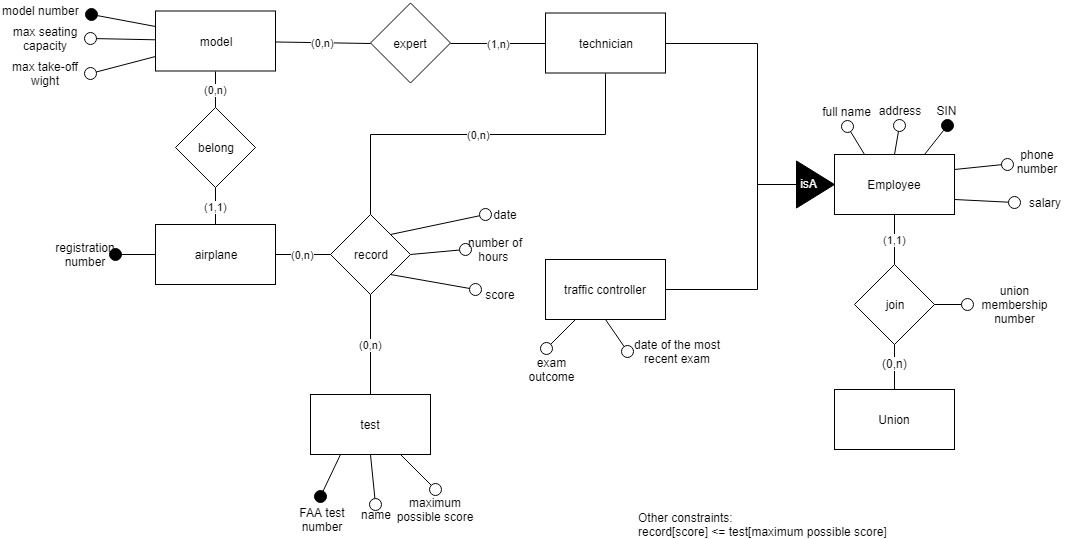
\includegraphics[scale=0.5]{3432.png}
\end{wrapfigure}
\end{enumerate}

\end{document}
